\documentclass[10pt,a4paper,onecolumn]{article}

\usepackage[utf8]{inputenx}
\usepackage[T1]{fontenc}
\usepackage{lmodern}
\usepackage{listings}
\usepackage{textcomp}
\usepackage[english,italian]{babel}
\usepackage{amsmath}
\usepackage{booktabs}
\usepackage{graphicx}
\usepackage[font=small,labelfont=bf,labelsep=period,tableposition=top]{caption}
\usepackage{tabularx}
\usepackage{multirow}
\usepackage{longtable}
\usepackage{fancyhdr}
\usepackage{lastpage}    
\usepackage{color}
\usepackage{enumitem}

\fancyhead{}
\renewcommand{\headrulewidth}{1pt}

\fancyhead[RE,RO]{
\begin{picture}(-135,0)
	%TODO \put(-482,-14){
\includegraphics[width=0.26\textwidth]{logoHead.png}} non sono molto bravo con gli strumenti grafici... qualcuno può creare un mini logo da collocare in questa posizione... l'idea è fare la scritta "Progetto di TecWeb... magari a destra di un simbolo che possa rappresentare internet... come... booo.. un mondo con un a rete attorno.... oppure un agglomerato dei loghi di browser come quella che ho scaricato!
	\put(-475,0){\sffamily\large\leftmark}
\end{picture}
}

\cfoot{}

\fancyfoot[RO,LE]{\sffamily Pag.~\thepage{} di \pageref{LastPage}} 
\fancyfoot[RE,LO]{Il mondo di Babe}

\renewcommand{\footrulewidth}{.2pt}
\pagestyle{fancy}

\renewcommand{\sectionmark}[1]{\markboth{#1}{#1}} 

% **************************************************
% Cross-references e collegamenti ipertestuali
% **************************************************
\usepackage[hidelinks]{hyperref}
\hypersetup{%
  colorlinks=false, linktocpage=false, pdfborder={0,0,0}, pdfstartpage=1, pdfstartview=FitV,%
  urlcolor=Cyan, linkcolor=Cyan, citecolor=Black, %pagecolor=Black,
  pdfcreator={pdflatex}, pdfproducer={pdflatex with hyperref package}%
}

\definecolor{dkgreen}{rgb}{0,0.6,0}
\definecolor{gray}{rgb}{0.5,0.5,0.5}
\definecolor{mauve}{rgb}{0.58,0,0.82}
 
\lstset{ %
  language=java,                % the language of the code
  basicstyle=\footnotesize,           % the size of the fonts that are used for the code
  numbers=left,                   % where to put the line-numbers
  numberstyle=\tiny\color{gray},  % the style that is used for the line-numbers
  stepnumber=2,                   % the step between two line-numbers. If it's 1, each line 
                                  % will be numbered
  numbersep=5pt,                  % how far the line-numbers are from the code
  backgroundcolor=\color{white},      % choose the background color. You must add \usepackage{color}
  showspaces=false,               % show spaces adding particular underscores
  showstringspaces=false,         % underline spaces within strings
  showtabs=false,                 % show tabs within strings adding particular underscores
  frame=single,                   % adds a frame around the code
  rulecolor=\color{black},        % if not set, the frame-color may be changed on line-breaks within not-black text (e.g. comments (green here))
  tabsize=2,                      % sets default tabsize to 2 spaces
  captionpos=b,                   % sets the caption-position to bottom
  breaklines=true,                % sets automatic line breaking
  breakatwhitespace=false,        % sets if automatic breaks should only happen at whitespace
  title=\lstname,                   % show the filename of files included with \lstinputlisting;
                                  % also try caption instead of title
  keywordstyle=\color{blue},          % keyword style
  commentstyle=\color{dkgreen},       % comment style
  stringstyle=\color{mauve},         % string literal style
  escapeinside={\%*}{*)},            % if you want to add LaTeX within your code
  morekeywords={*,...},              % if you want to add more keywords to the set
  deletekeywords={...}              % if you want to delete keywords from the given language
}

% **************************************************
% Macro
% **************************************************
\newcommand{\sitepage}[1]{\textcolor{cyan}{\textsf{#1}}}
\newcommand{\inglese}[1]{\foreignlanguage{english}{\itshape{}#1}}
\newcommand{\progname}[1]{\textcolor{blue}{\textsf{#1}}}

\begin{document}
%----------------------------------------------------------
\begin{titlepage}

\begin{center}
% Upper part of the page
 
\textsc{\Large}\\[5cm]


\includegraphics[width=0.4\textwidth]{Logo.png}\\[0.3cm]  
\noindent\rule{\textwidth}{0.4pt} \\[0.3cm]
\textsc{\Huge Progetto di}\\[0.25cm]
\textsc{\Huge Tecnologie Web}\\[0.3cm]
\textsc{\Large Sito ``Il mondo di Babe''}
\noindent\rule{\textwidth}{0.4pt}\\[0.5cm]
\textit{``Sviluppare un sito accessibile secondo gli standard web''} \\[0.5cm]
\textsc{20 febbraio 2013}\\[0.5cm]
\begin{minipage}{0.4\textwidth}
\begin{flushleft} \large
\emph{Studente:}\\
Andrea Meneghinello\\
Andrea Rizzi\\
Diego Beraldin\\
Elena Zecchinato
\end{flushleft}
\end{minipage}
\begin{minipage}{0.4\textwidth}
\begin{flushright} \large
\emph{Matricola:} \\
610762\\
610761\\
1006523\\
1007584\\
\end{flushright}
\end{minipage}
\end{center}
\end{titlepage}
%-----------------------------------------------------------------------

\clearpage

\tableofcontents

\clearpage 

\begin{abstract}
Questo progetto consiste nella realizzazione di un sito che ha come protagonista il simpatico maialino Babe, personaggio principale dei film ``Babe maialino coraggioso'' e ``Babe va in città''.
Si tratta di un sito didattico che ha lo scopo di sensibilizzare i bambini sul tema degli animali facendoli immergere nel mondo di Babe, nella sua storia ed imparando con lui i primi rudimenti come i numeri e l'alfabeto, affinché possano amare fin da subito gli animali ed imparare il rispetto per questi ultimi.
\end{abstract}

\clearpage

\section{Analisi dei requisiti}
% chi sono i destinatari del sito, quali sono le loro necessita' e come le soddisfiamo
% font, colori, immagini
% sito pensato per lavagne interattive multimediali (LIM) per essere utilizzata negli asili

\subsection{Scelte per il posizionamento sui motori di ricerca}
Nella progettazione del sito, alcune scelte sono state dettate dall'esigenza di attuare strategie di ottimizzazione per i motori di ricerca.

In primo luogo è stata adottata una rigida separazione fra contenuto, comportamento e presentazione, separando su file diversi le istruzioni di formattazione (regole CSS) e il codice JavaScript.\footnote{%
  PERL non è incluso in questo elenco dal momento che la sua interpretazione lato server non implica che il contenuto degli script debba essere scaricato di volta in volta sui client.
} Tale decisione ha il duplice effetto di ridurre la dimensione complessiva delle pagine, dal momento che il codice è incluso in più documenti e viene scaricato una sola volta nonché di inviare ai motori di ricerca testo significativo rispetto al contenuto reale delle pagine.

In secondo luogo, si è scelto di aderire allo stanard XHTML versione 1.0 ``Strict'', utilizzando ovunque fosse possibile un \inglese{markup} semantico e strutturale, evitando l'impiego di tag presentazionali deprecati.


In terzo luogo, come sarà illustrato con maggiori dettagli nella sezione \ref{sec:accessibility}, si è scelto di rispettare le direttive WCAG per l'accessibilità delle pagine, in modo da rendere i contenuti fruibili anche in modalità alternative rispetto alla disposizione bidimensionale di contenuti e immagini su uno schermo, da cui sono esclusi tanto gli utenti diversamente abili quanto i \inglese{web spider} e i motori di ricerca.

Infine, si è posta particolare attenzione all'utilizzo dei tag \texttt{<meta>}, in particolare \texttt{description}, \texttt{keywords} e \texttt{rating}. È stata infatti inserita una descrizione significativa specifica per ogni singola pagina, pensata per essere accattivante se visualizzata in una SERP (\inglese{search engine response page}).

Le parole chiave sono state selezionate in modo specifico per ogni pagina, scegliendo tra i termini che compaiono nelle posizioni più ``prominenti'' (intestazioni, elenchi, collegamenti, enfasi) ed effettivamente presenti nel contenuto della pagina. Inoltre, il numero di parole chiave è stato mantenuto contenuto a un numero inferiore a dieci.

La valutazione del contenuto di tutte le pagine è stata impostata a \texttt{safe for kids}, una scelta le cui ragioni sono da ravvisarsi nel fatto che il sito ha una finalità didattica per bambini, e quindi gli autori hanno tutto l'interesse a presentare contenuti sicuri e adatti al pubblico dei più piccoli.

\section{Design architetturale}
% quale schema organizzativo e' stato scelto, come sono state organizzate le informazioni
\subsection{Schemi organizzativi}
Il contenuto delle pagine è organizzato secondo uno schema ambiguo, in particolare lo schema organizzativo per argomento (\inglese{topical}).

Ad esempio, nella pagina \sitepage{ImparaConBabe.html}, che contiene le schede didattiche, gli argomenti in cui è organizzato il contenuto sono:
\begin{itemize}[noitemsep,nolistsep]
  \item[-] l'alfabeto;
  \item[-] i numeri;
  \item[-] i colori;
  \item[-] i giorni della settimana;
  \item[-] i mesi;
  \item[-] le stagioni.
\end{itemize}

Per quanto riguarda la disposizione degli elementi nelle singole pagine, la scelta di organizzazione dei contenuti è ricaduta sul modello di \inglese{layout} <<a tre pannelli>>. Tale modello prevede la ripartizione delle informazioni tra l'intestazione, il menu di navigazione e il contenuto centrale, che rispondono rispettivamente ai quesiti `Dove sono?', `Dove posso andare?' e `Di cosa si tratta?'.

\subsection{Strutture organizzative}
Il modello di navigazione utilizzato ad alto livello è lo schema gerarchico. Tale struttura è stata scelta al fine di permettere all'utente di crearsi con facilità una mappa mentale del sito ed evitare in tal modo il disorientamento. In particolare, si è evitato di rendere la gerarchia troppo estesa in ampiezza, limitando il numero di voci totali a sette.

Nei livelli sottostanti della gerarchia si è invece adottata la struttura organizzativa di tipo ipertestuale ma con possibilità di spostamento solo all'interno delle singole pagine. In tal modo si è permessa una maggiore flessibilità di navigazione evitando però l'insorgenza di difficoltà nella creazione della mappa mentale da parte dell'utente.

Pur essendo il sito orientato alla didattica, non si è ritenuta necessaria l'adozione di una struttura organizzativa sequenziale perché gli insegnamenti impartiti sono talmente basilari e scorrelati gli uni dagli altri da non necessitare l'imposizione di un percorso obbligato.

\subsection{Layout delle pagine}
Per quanto riguarda il \inglese{design} delle pagine, la scelta per il dimensionamento degli elementi è stata la creazione di un \inglese{layout} fluido, in grado di adattarsi alle dimensioni (in particolare sull'asse orizzontale) dello schermo. Ovunque fosse possibile le misure sono state espresse in unità relative, come le percentuali tanto per la dimensione dei contenitori di testo quanto per le immagini.

% TODO spiegare come è stato ottenuto l'effetto dello sfondo a parallasse

Inoltre, come specificato nella sezione \ref{sec:testoaccessibile} per le parti testuali si è deciso di adottare una misura relativa espressa in \texttt{em} in modo da rispettare per quanto possibile le preferenze impostate dall'utente e ottenere quindi un certo grado di elasticità nel \inglese{layout} delle pagine.

In relazione al supporto ai caratteri, si è scelto di utilizzare nel foglio di stile la direttiva
\begin{verbatim}
  font-family: Verdana, Helvetica, sans-serif;
\end{verbatim}
in modo da assicurare una visualizzazione simile su ogni dispositivo indipendentemente dal sistema operativo e dai font tipografici supportati.

Per assicurare un buon grado di uniformità nella visualizzazione dei colori si sono utilizzati esclusivamente colori \inglese{web-safe} vale a dire i colori che nella loro rappresentazione esadecimale contengono solo le cifre \verb+0+, \verb+3+, \verb+6+, \verb+9+, \verb+c+ e \verb+f+.

Per garantire una trasformazione elegante del \inglese{layout} in tutte le circostanze e, in particolare:
\begin{enumerate}[noitemsep,nolistsep,label=\emph{\alph*})]
  \item\label{item1} in caso di ridimensionamento della finestra del browser;
  \item\label{item2} in caso di visualizzazione su dispositivi con schermo di dimensioni ridotte;
  \item\label{item3} nel caso in cui l'utente abbia impostato una dimensione dei caratteri molto grande;
\end{enumerate}
è stata impostata l'attivazione del CSS \texttt{SmallLayout.css} con una misura relativa in \texttt{em}. Utilizzando infatti nell'elemento \texttt{<link>} una misura dello schermo espressa in pixel si garantisce la trasformazione per tutti i browser per i soli casi \ref{item1} e \ref{item2} mentre l'attivazione del CSS alternativo nel caso \ref{item3} avviene solo in alcuni browser (es. Firefox).

\section{Mappa del sito}
\begin{figure}[tb]
\centering
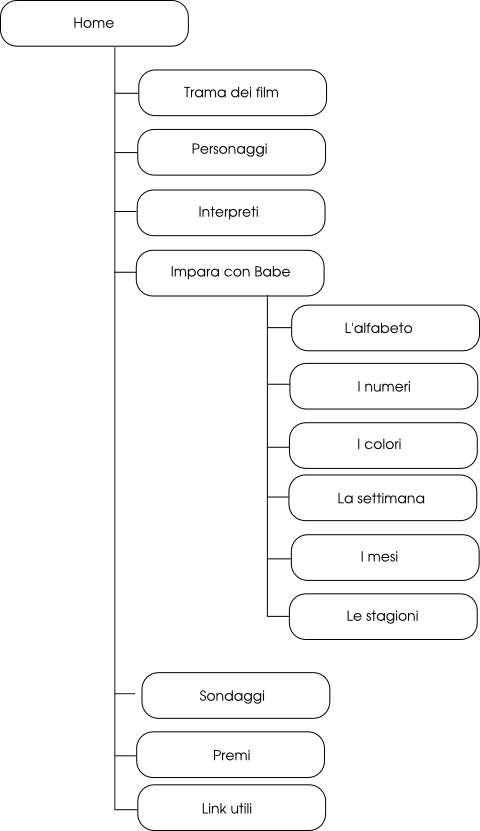
\includegraphics[width=.8\textwidth]{mappasito.png}
\caption{Organizzazione delle pagine del sito}
\end{figure}

\clearpage

\section{Accessibilità}\label{sec:accessibility}

\subsection{Il testo}\label{sec:testoaccessibile}
Per quanto riguarda il testo si è cercato di fare particolare attenzione alla dimensione e ai font utilizzati. Infatti, essendo un sito per bambini è bene avere un testo facilmente leggibile sia in relazione alla dimensione che ai font utilizzati.

Non si sono infatti impiegati font particolari e le dimensioni del testo sono assegnate con il parametro \texttt{em} che permette l'adattamento del testo in base alle caratteristiche desiderate dall'utente.  

Si è inoltre cercato di utilizzare un linguaggio il più chiaro possibile visto che il pubblico a cui ci si rivolge sono i bambini è ancor più importante essere chiari e semplici.

Infine, laddove possibile, si è fatto uso di strutture enumerative (liste ordinate o non ordinate) per presentare le informazioni in forma schematica e più facilmente accessibile in quanto già strutturata e non ``appiattita'' in forma testuale.

\subsection{I link}
Per quanto riguarda i link si è deciso di non rompere le convenzioni esterne evitando di personalizzarne l'aspetto all'interno del sito.
In questo modo l'utente non è in alcun modo indotto in errore. Considerando che il nostro target può essere potenzialmente un utente con poca esperienza si è preferito mantenere la convenzione standard sui link.

In particolare nella pagina \sitepage{ImparaConBabe.html} sono usate delle immagini per anticipare all'utente il contenuto della pagina di destinazione del link.
Le immagini costituiscono un link insieme al testo  e perciò la zona su cui è necessario cliccare per accedere alle pagine è sufficientemente ampia da poter essere accessibile anche dalle persone che hanno difficoltà nel muovere il mouse.

All'interno del sito sono presenti dei link esterni, in questo caso si è segnalato esplicitamente tramite l'immagine di un mondo che il link porta all'esterno del sito (ad esempio \sitepage{Stagioni.html}). Tale convenzione interna è stata mantenuta per tutte le pagine in cui comparivano dei collegamenti esterni, con il preciso intento di non deludere le aspettative dell'utente.

Le pagine di dimensione verticale maggiore, ad esempio \sitepage{Alfabeto.html}, \sitepage{Mesi.html} o \sitepage{Trama.html} contengono inoltre dei collegamenti interni per tornare in cima alla pagina durante la navigazione. La pagina dei \sitepage{Personaggi.html}, oltre a questo tipo di collegamenti, permette di spostarsi da un personaggio all'altro durante la lettura. La pagina \sitepage{Mesi.html} contiene una filastrocca sui mesi che contiene un collegamento per ogni mese. La stessa cosa avviene per la pagina \sitepage{Giorni.html}, che contiene però una filastrocca sui giorni, con relativi collegamenti. Si è utilizzata tale tecnica solo con il fine di presentare la pagina in modo simpatico e permettere di muoversi liberamente all'interno delle pagine.



Per rendere più rapida la navigazione si è scelto di offrire la possibilità di saltare gli elementi che esulano dal contenuto in senso stretto, quali il menu di navigazione o la lista dei \inglese{feed RSS} che si ripetono uguali in ogni pagina e che dunque non necessitano di essere letti ogni volta. A tal fine, sono stati inseriti dei collegamenti nascosti (impostando una posizione assoluta che ecceda il margine sinistro), che però risultano accessibili se si legge il solo contenuto testuale della pagina.

Si è inoltre prestata particolare attenzione a evitare la presenza di link circolari, a rendere il testo delle ancore facilmente individuabile e, soprattutto, sufficientemente autoesplicativo riguardo alla posizione di destinazione (evitando accuratamente di utilizzare parole ``vuote'' o deittici come testo dei link).
Inoltre, si è fatta attenzione a non rendere i link presenti nella \inglese{breadcrumbs}\footnote{%
   \inglese{Breadcrumbs} significa letteralmente ``briciole di pane''. Si tratta di una tecnica utilizzata per aiutare l'utente a non perdersi all'interno del sito, fornendogli le traccie del percorso esplorativo da lui effettuato, proprio come Pollicino aveva lasciato le briciole di pane nel bosco per poter ritrovare la strada di casa.}adiacenti, separandoli tramite il carattere ``>''

Per facilitare la navigazione fra le pagine attraverso i collegamenti ipertestuali è stato impostato l'attributo \texttt{tabindex} per i link del menu principale e delle \inglese{breadcrumbs}, nonché per il collegamento `Salta al contenuto' che non è direttamente visibile sulle pagine.

Si è scelto invece di non inserire alcuna \inglese{access key} perché sarebbe stato difficile trovare delle combinazioni da tastiera non già assegnate dalle applicazioni o dagli ambienti desktop e, inoltre, perché si è valutato il sito sufficientemente navigabile anche senza questa opzione.

\subsection{Le immagini}
Nel sito le immagini sono molto numerose, essendo infatti un sito per bambini molte cose sono spiegate con l'aiuto di immagini. La dimensione delle immagini è stata mantenuta sotto controllo e, ove necessario, sono state ridimensionate per consentire una migliore visualizzazione senza appesantire eccessivamente il caricamento della pagina.

Per ogni immagine è stata valutata la necessità di inserire del testo nell'attributo \texttt{alt} per permettere allo \inglese{screen reader} di descrivere l'immagine o di poter visualizzare il testo alternativo qualora l'immagine non si potesse vedere. Le descrizioni inserite sono sufficientemente esplicative ma di breve lunghezza, in modo che la loro lettura non richieda un tempo eccessivo.\footnote{%
    L'uso dell'attributo \texttt{longdesc} per inserire descrizioni più lunghe è stato giudicato inopportuno dato il suo scarso supporto da parte dei browser.
}

Nella pagina \sitepage{ImparaConBabe.html} le immagini servono solo per dare all'utente un'idea del contenuto della pagina che andranno ad aprire, perciò si è deciso di non mettere il testo alternativo. 
Nella pagina \sitepage{Alfabeto.html} si è deciso di non commentare gli \texttt{alt} in quanto il testo presente è sufficientemente descrittivo e la presenza di testo nell'attributo \texttt{alt} risulterebbe superflua.
Si è fatta una scelta analoga per la pagina dei colori, dove si è ritenuto il contenuto testuale sufficiente anche senza la presenza del testo alternativo.

Anche per la pagina dei giorni si è scelto di non inserire il testo alternativo visto che le immagini sono la rappresentazione della filastrocca e quindi descriverle sarebbe inutile.
Qualora le immagini per qualche motivo non fossero visualizzabili questo non inciderebbe in alcun modo sul contenuto della pagina.

Per la pagina dei numeri invece si è scelto di descrivere le immagini.
La ragione principale risiede nel fatto che, qualora le immagini non fossero visualizzabili il testo non sarebbe sufficiente a garantire la consistenza del contenuto in quanto si potrebbero leggere solo i numeri in lettere ma non in cifre.

Per la pagina \sitepage{Stagioni.html} si è scelto di inserire del testo nell'attributo \texttt{alt}. Le immagini scelte, infatti,  rappresentano simbolicamente le stagioni perciò si è ritenuto giusto riportare un testo alternativo.
Una scelta analoga si è fatta per la pagina \sitepage{Mesi.html}, in quanto ogni immagine riportata rappresenta simbolicamente un mese.

\subsection{Il colore}
In generale, la tavolozza dei colori adottata per la realizzazione delle pagine è basata sui colori caldi (rosa, arancio, legno chiaro) e intende rimandare ai colori della fattoria e del mondo agreste da cui provengono i personaggi degli sceneggiati che hanno come protagonista Babe.

La scelta dei colori è stata guidata dal duplice scopo di ottenere una serie di pagine esteticamente gradevoli anche in vista del pubblico di bambini ma anche, al tempo stesso, di garantire un adeguato contrasto dei colori per gli utenti affetti da patologie in grado di alterare la percezione cromatica.

In ogni caso, nella scelta dei colori, qualora vi fosse un conflitto fra l'estetica delle pagine e l'accessibilità, si è sempre preferito salvaguardare la seconda, anche in relazione all'esito dei test sui colori che sono stati realizzati con gli strumenti descritti nella sezione \ref{sec:strumenti}.

\subsection{I form}
I form che compaiono nella sezione \sitepage{Sondaggi.html} del sito sono stati progettati e realizzati al fine di massimizzare l'accessibilità. In primo luogo, tutti gli elementi \texttt{<input>} sono stati inseriti all'interno di un elemento \texttt{<fieldset>} corredato da un'opportuna \texttt{<legend>}, in modo da rendere evidente la suddivisione logica nelle varie sezioni del contenuto.

In secondo luogo, tutti gli elementi \texttt{<input>} sono corredati dalla rispettiva \texttt{<label>} che permette di associare un'etichetta informativa relativamente alla tipologia di valori attesi dal campo di inserimento, semplificando l'interazione con l'utente anche nel caso in cui questi ricorra all'uso di tecnologie di accesso universale.

%TODO tabindex
%TODO aiuti per dati inseriti erroneamente
%TODO title

\subsection{Le tabelle}
Le tabelle che compaiono nella sezione \sitepage{Interpreti.html} sono state progettate per essere fruibili anche in forma non visuale, mediante l'utilizzo dell'attributo \texttt{scope} rispettivamente con il valore \texttt{col} per le intestazioni delle colonne e con il valore \texttt{row} per la testata di ogni riga, ovvero il personaggio di cui si elencano gli attori della versione originale e i doppiatori della versione italiana.

Tramite un simile accorgimento, chi accede al contenuto del sito mediante un sintetizzatore vocale potrà sentire prima del contenuto di ogni cella l'indicazione del personaggio a cui si riferisce l'informazione (che corrisponde all'indice di riga) e il ruolo che viene presentato (che corrisponde alla colonna) anche in assenza delle informazioni che normalmente vengono veicolate dalla disposizione spaziale del testo.

L'organizzazione delle informazioni nella tabella è resa ancor più chiara dall'attributo \texttt{summary}, in cui oltre a giustificare la suddivisione in righe e colonne è illustrato brevemente il contenuto della tabella, in modo tale che chi accede al contenuto tramite uno \inglese{screen reader} possa saltare il contenuto qualora non interessato.

Al fine di utilizzare un \inglese{markup} quanto più semantico possibile, inoltre, in ognuna delle due tabelle si è fatto ricorso a un elemento \texttt{<thead>} per creare le intestazioni delle tre colonne, in cui sono stati inseriti come figli di secondo livello degli elementi \texttt{<th>}. L'utilizzo di un \inglese{footer} non è invece stato ritenuto necessario, dal momento che il numero di righe è piuttosto ridotto (otto nella tabella degli interpreti e dieci in quella delle voci degli animali). Infine, come ultimo accorgimento per agevolare la lettura, si è scelto di alternare i colori delle righe adiacenti.

\subsection{Accorgimenti per gli screen reader}
In tutte le pagine, le parole che comparivano in lingue diverse da quella principale sono state inserite all'interno di un elemento in cui è specificato l'attributo \texttt{xml:lang}, eventualmente aggiungendo uno \texttt{<span>} qualora la porzione di testo interessata non fosse già racchiusa in un elemento superiore.

In tal modo gli \inglese{screen reader} saranno in grado di adottare la pronuncia corretta, in special modo per i numerosi nomi dei personaggi che hanno mantenuto il nome originale anche nella versione doppiata dei film.

Inoltre, ancora una volta allo scopo di facilitare la fruizione del contenuto a chi accede al sito tramite tecnologie di sintesi vocale, le eventuali sigle o abbreviazioni, ad esempio ``RSS'' sono stati inseriti all'interno di un elemento \texttt{<abbr>} in cui tramite l'attributo \texttt{title} si fornisce la dicitura per esteso.
\subsubsection{Risconti sui test effettuati con gli screen reader}
Al fine di garantire l'accessibilità al sito, in particolare per le persone con disabilità visive, si sono effettuati dei test con due  \inglese{screen reader} differenti. 
Si è volta particolare attenzione al controllo della fruibilità di:
\begin{itemize}[noitemsep,nolistsep]
  \item[-] menu;
  \item[-] tabelle;
  \item[-] immagini;
  \item[-] pronunce linguistiche corrette;
\end{itemize}

Per quanto riguarda il menu, si è controllato che lo \inglese{screen reader} accedesse al menu secondo l'ordine stabilito e che legga in particolare la voce salta menu, non visibile direttamente nella pagina ma fondamentale per le persone con problemi visivi, che altrimenti sarebbero costrette ad una forzata rilettura delle voci del menu per ogni accesso alle pagine. Il riscontro in questo caso è stato positivo.

Per quanto riguarda le tabelle si è controllato che lo \inglese{screen reader} leggesse correttamente le intestazioni di riga e di colonna prima di leggere il contenuto delle celle. Purtroppo tale riscontro non ha avuto esito positivo. Tuttavia, avendo seguito tutte le regole per ottenere tabelle accessibili, si ritiene che l'esito negativo del test derivi dal fatto che gli screen-reader utilizzati sono strumenti gratuiti e di conseguenza probabilmente non godono di tutte le funzionalità.

Per quanto riguarda invece le immagini, i test hanno avuto un riscontro positivo. Si è controllato che lo \inglese{screen reader} leggesse il valore degli attributi \texttt{alt} dove presente. Inoltre si è cercato di capire tramite l'uso di \inglese{screen reader} se il contenuto del sito senza la visione di immagine fosse mantenuto.

Per quanto riguarda la correttezza nella pronuncia di parole appartenenti ad altre lingue, purtroppo il test ha dato esito negativo. Entrambe gli \inglese{screen reader} utilizzati non distinguono il cambiamento di lingua impostato tramite l'attributo  \texttt{xml:lang}.  Anche in questo caso si pensa che la colpa sia del fatto che gli strumenti utilizzati sono gratuiti.

\section{Note}
\subsection{Note sulle pagine Mesi e Giorni}
Il contenuto della pagina viene presentato servendosi di una filastrocca. La struttura della filastrocca richiede che ogni verso occupi una riga differente. Per fornire questa struttura si è inserito ogni verso in un tag \texttt{<p>}.

Si è scelto di non usare il tag \texttt{<pre>} in quanto pur garantendo la conservazione di spazi e ritorni a capo, tale tag rende più complessa la manipolazione per il ridimensionamento della pagina.

Infatti usando il tag \texttt{<pre>} viene disabilitato il ritorno a capo automatico e perciò se la pagina diventa troppo piccola il testo esce della pergamena posta come sfondo.

\subsection{Note sul titolo}

Per quanto riguarda il titolo, si è scelto di non utilizzare tecniche di \inglese{image replacement}, penalizzando così la grafica, per mantenere l'accessibilità. Le tecniche di \inglese{image replacement} anche se sono in grado di permettere al sito di avere una buona grafica pur mantenendo un certo grado di accessibilità, comunque la penalizzano in qualche modo. Infatti, utilizzando tali tecniche si dovrebbe rinunciare o ad un buon ridimensionamento oppure alla sicurezza assoluta che sia conservato il contenuto in quanto se le immagini dovessero essere disabilitate allora non si potrebbe più leggere il titolo e di conseguenza non si potrebbe più rispondere alla domanda ``dove sono?''. Quindi, si è scelto di avere un titolo non pienamente appagabile dal punto di vista estetico ma che fornisce una sicurezza nel suo mantenimento.

\section{Strumenti ultilizzati}\label{sec:strumenti}

Il programma \progname{Totalvalidator}, in versione gratuita, è stato utilizzato per verificare il rispetto delle linee guida WCAG 2.0, ottenendo la valutazione AA2.


Gli \inglese{screen reader}  \progname{	NVDA} e  \progname{Orca} sono stati utilizzati per verificare l'accessibilità al contenuto da parte di utenti con disabilità visive.

Lo strumento \progname{Color Oracle} è stato utilizzato al fine di simulare la visione di un utente affetto da dicromatismo, vale a dire un soggetto in cui solo due tra le tre normali discriminazioni visive (luce/buio, giallo/blu e rosso/verde) sono presenti, in particolare:

\begin{tabular}{>{\sffamily\bfseries}lp{.7\textwidth}}
  Deuteranopia: & per cui il color rosso porpora è indistinguibile dal verde\\
  Protanopia: & ossia l'incapacità di percepire il colore rosso\\
  Tritanopia: & ovvero la cecità per i colori blu e violetto\\
\end{tabular}

Alcuni test specifici per l'accessibilità (ad esempio il contrasto dei colori) sono stati portati a termine con lo strumento \progname{JuicyStudio}. Grazie a questo strumento è stato possibile verificare per ogni pagina, e per ogni elemento contenuto in ogni pagina, un'analisi di contrasto relativamente a:
\begin{itemize}[noitemsep,nolistsep]
  \item[--] rapporto luminosità/contrasto;
  \item[--] differenza di luminosità;
  \item[--] differenza di colore.
\end{itemize}

I risultati ottenuti sono compresi, rispettivamente, tra 9.4 : 1 e 21:1, tra 207 e 255 nel secondo caso e tra 527 e 765 nel caso del terzo parametro. Tali valori sono stati considerati accettabili in quanto superiori alle soglie minime di 7:1 per il rapporto luminosità/contrasto, 125 per la differenza di luminosità e 500 per la differenza di colore, rientrando dunque con ampio margine nella categoria di accessibilità AA\@.

Infine, utilizzando l'estensione \progname{Accessibility Evaluation Tool} per Firefox è stato possibile testare la visualizzazione delle varie pagine rimuovendo il CSS definito dall'utente, con contrasto elevato (B/W e W/B), rimuovendo le immagini di sfondo, le immagini di contenuto o tutte le immagini al fine di constatare la fruibilità dei contenuti anche in contesti diversi da quello di usuale visualizzazione. Tramite il browser testuale \progname{w3m} è stata inoltre testata la navigabilità del sito in modalità solo testo. 

\section{Pagine dinamiche}

\subsection{Utilizzo XML}

\subsection{Utilizzo Perl}

\clearpage

\section{Norme di sviluppo}

\subsection{Norme di sviluppo XML}

\subsection{Norme di sviluppo CSS}

Il sito basa la gestione del proprio layout grafico su due fogli di stile CSS: NormalLayout.css e SmallLayout.css. Il primo viene usato per gestire una normale visione su schermo avente una larghezza superiore a 52em. Il secondo foglio invece si occupa di adattare la pagina nel momento in cui questa raggiunge una larghezza inferiore a 52em, e viene caricato sui dispositivi mobile. Nel progettare e sviluppare tali CSS si sono tenute in considerazione le seguenti norme:

\begin{itemize}
  \item Privilegiare il contenuto del sito, sacrificando (nel caso) alcuni effetti CSS ``accattivanti'' ma che penalizzano la lettura del contenuto.
  \item Mai usare CSS embedded o inline, ma creare file CSS da richiamare mediante link nel documento html.
  \item Al termine di ogni modifica significativa, ripetere il test di validazione del W3C.
  \item Mai abusare degli elementi <div>. È giusto crearli per evidenziare la presenza di una ``regione semantica'' rilevante, o nel caso che il layout grafico richieda particolari effetti flottanti, ma si esorta i componenti a non usarlo la dove possibile.
  \item Nel scegliere i nomi da dare alle classi, tenere in considerazione che tali dovrebbero esprimere il significato dell'oggetto su cui si applicherà, e non le caratteristiche di visualizzazione poiché tali sono mutevoli e potrebbero cambiare in futuro (e.g. se si intende rappresentare una <label> con una certa colorazione, non si dovrà chiamare .labelRossa, ma bensì .etichetta, presupposto il fatto che ci interessa rappresentarla come un etichetta che contraddistingue un determinato <input>).
\end{itemize}

\subsubsection{Versione CSS}
Nello sviluppo del CSS si sono utilizzate alcune proprietà che esulano dalla versione 2.1 dello standard, in particolare \verb+border-radius+ e \verb+background-size+.

La visualizzazione del sito è stata comunque testata con browser che non supportano le regole CSS3 (non ancora standard) e il risultato ottenuto, seppur non esteticamente gradevole come nei browser più recenti, conserva il contenuto.

\clearpage

\section{Riferimenti bibliografici e materiale di consultazione online}

\end{document}


